\documentclass{article}
\usepackage{fancyhdr} % Required for custom headers
\usepackage{lastpage} % Required to determine the last page for the footer
\usepackage{extramarks} % Required for headers and footers
\usepackage{graphicx} % Required to insert images
%\usepackage{lipsum} % Used for inserting dummy 'Lorem ipsum' text into the template
\usepackage{amsmath}
%\usepackage{amsfont}
%\usepackage{amssymb}

\usepackage{multicol}
% Margins
\topmargin=-0.5in
\evensidemargin=0in
\oddsidemargin=-0.5in
\textwidth=7.5in
\textheight=9.0in
\headsep=0.25in 


\pagestyle{fancy}

\rhead{M. Adam} % Top right header
\lhead{Sweet Pea Salad}
\chead{ }
%\title{}

\begin{document}
%
%PRELIMINARIES:
%
%
%Begin by preheating the oven to 350 $^o$F
%
%\bigskip
%
%\bigskip

\begin{multicols}{2}
Ingredients:
\begin{itemize}
\item 4 cups of fresh shelled English peas (also known as shelling peas or garden peas)
\item 3-4 green onions (scallions), finely chopped
\item 1/3 cup of crumbled sheep's milk cheese
\item 2 tbsp of olive oil
\item 1 tsp of fresh lemon juice
\item 1/4 cup of finely chopped Kalamata olives
\item 1 pinch of grated lemon rind
\item Salt and pepper to taste
\end{itemize}

\columnbreak

Directions:
\begin{enumerate}
\item In a saucepan bring approx. 1 inch (2.5 cm) of water to a boil and lower in the steamer basket. While the water is coming to a boil, shell the peas and chop the onions.

\item Allow the peas to steam over boiling water in the steamer basket for approx. 2 minutes.

\item Remove the peas from the steamer and immerse in an ice-water bath to stop the cooking process. Then strain the peas.

\item Transfer the peas into a salad bowl, add the olives, feta cheese, onions, olive oil, lemon juice, lemon rind, and salt and pepper to taste.

\item Toss them all together and enjoy!

\end{enumerate}
\end{multicols}



\begin{center}
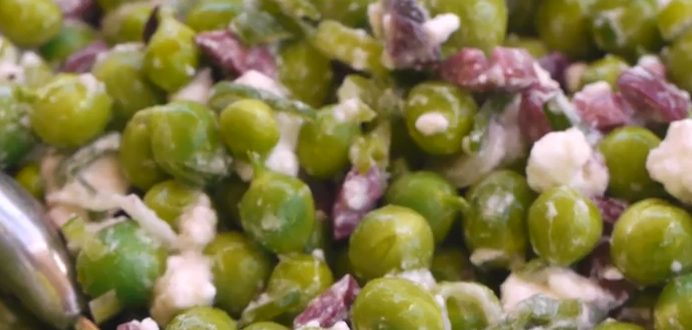
\includegraphics[scale=0.4]{SweetPeaSalad.png}
\end{center}


\end{document} 











